\documentclass[a4paper, 14pt]{extarticle}%тип документа

%Русский язык
\usepackage[T2A]{fontenc} %кодировка
\usepackage[utf8]{inputenc} %кодировка исходного кода
\usepackage[english,russian]{babel} %локализация и переносы

%отступы 
\usepackage[left=2cm,right=2cm,top=2cm,bottom=3cm,bindingoffset=0cm]{geometry}

%Вставка картинок
\usepackage{graphicx}
\usepackage{wrapfig, caption}
\graphicspath{}
\DeclareGraphicsExtensions{.pdf,.png,.jpg, .jpeg}
\newcommand\ECaption[1]{%
     \captionsetup{font=footnotesize}%
     \caption{#1}}

%Таблицы
\usepackage[table,xcdraw]{xcolor}
\usepackage{booktabs}

%Графики
\usepackage{pgfplots}
\pgfplotsset{compat=1.9}

%Математика
\usepackage{amsmath, amsfonts, amssymb, amsthm, mathtools}

%Заголовок
\author{Подлесный Артём \\ группа 827}
\title{Работа 4.2 \\ Исследование энергетического спектра $\beta$-частиц и определение их максимальной энергии при помощи магнитного спектрометра.}

\begin{document}
\maketitle

\section*{Краткая теория}

В данной работе рассматривается электронный распад:
\begin{equation}
_Z^AX \to _{Z+1}^AX+e^-+\widetilde{\nu}.
\end{equation}

\begin{wrapfigure}{r}{0.3\textwidth}
\begin{center}
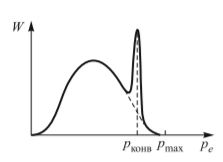
\includegraphics[height=4cm]{1.png}
\end{center}
\ECaption{Форма спектра $\beta$-частиц при разрешенных переходах.}
\end{wrapfigure}
Из этого уравнения можно получить распределения количества частиц $dN$ в промежутке с абсолютным значением импульсов между $p$ и $p+dp$:
\begin{equation}
dN = \frac{16\pi^2N_0}{c^2}Dp^2(E_e - E)^2dp.
\end{equation}

При переходе от $dp$ к $dE$ получаем:
\begin{equation}
dE = \dfrac{c^2p}{E+mc^2}dp.
\end{equation}

Отсюда получаем функцию спектра на рис 1:
\begin{equation}
W = \dfrac{dN}{dE} \approx \sqrt{E}(E_e-E)^2.
\end{equation}

Дочерние ядра, образующиеся при $\beta$-распаде, если они оказываются возбужденными, успускают $\gamma$-квант, который передает избыток энергии электронам с оболочек атомов. Излучаемые таким образом электроны имеют определенную энергию и называются конверсионными. 

\section*{Экспериментальная установка}

\begin{figure}[h]
\begin{center}
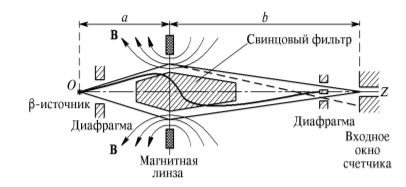
\includegraphics[width=0.9\textwidth]{ust}
\ECaption{Схема $\beta$-спектрометра.}
\end{center}
\end{figure}

Исходя из принципов работы спектрометра можем получить такие соотношения для экспериментальных данных:
\begin{equation}
p_e = kI,
\end{equation}
\begin{equation}
 N(p_e) = CW(p_e)p_e,
\end{equation}
где $k$ и $C$ -- некоторые константы.

\section*{Обработка экспериментальных данных}
 
Измерения проводились для 32 значений тока в промежутке от 1 до 5 А. Каждое измерение проводилось с интервалом в 100 секунд. Полученные результаты представлены на таблице 1.
\begin{table}[h!]
\begin{center}
\begin{tabular}{|c|c|c|c|}
\hline
\rowcolor[HTML]{6665CD} 
$I$, A & $N$, $c^{-1}$ & $I$, A & $N$, $c^{-1}$ \\ \hline
0.3    & 0.53          & 4      & 1.72          \\ \hline
\rowcolor[HTML]{CBCEFB} 
0.6    & 0.67          & 4.05   & 3.109         \\ \hline
0.9    & 0.96          & 4.1    & 7.078         \\ \hline
\rowcolor[HTML]{CBCEFB} 
1      & 1.33          & 4.15   & 12.476        \\ \hline
1.2    & 1.909         & 4.2    & 11.447        \\ \hline
\rowcolor[HTML]{CBCEFB} 
1.5    & 1.3989        & 4.25   & 12.126        \\ \hline
1.8    & 6.318         & 4.3    & 12.926        \\ \hline
\rowcolor[HTML]{CBCEFB} 
2      & 9.867         & 4.35   & 12.876        \\ \hline
2.1    & 8.188         & 4.4    & 9.267         \\ \hline
\rowcolor[HTML]{CBCEFB} 
2.4    & 9.377         & 4.45   & 4.409         \\ \hline
2.7    & 9.247         & 4.5    & 3.109         \\ \hline
\rowcolor[HTML]{CBCEFB} 
3      & 7.818         & 4.6    & 1.52          \\ \hline
3.3    & 4.829         & 4.7    & 0.62          \\ \hline
\rowcolor[HTML]{CBCEFB} 
3.5    & 3.259         & 4.8    & 0.36          \\ \hline
3.6    & 2.099         & 4.9    & 0.45          \\ \hline
\rowcolor[HTML]{CBCEFB} 
3.9    & 1.59          & 5      & 0.37          \\ \hline
\end{tabular}
\ECaption{Таблица с результатами эксперимента, зависимости $I(N)$ -- силы тока от среднего числа электронов в секунду.}
\end{center}
\end{table}

Так же был измерен фон при 0 токе перед и после проведения основных измерений. Он появляется преимущественно из-за $\gamma$-квантов и электронов, рассеянных от стенок спектрометра. По результатам измерений средний фон равен:
\[N_{\text{Ф}} = 0.61 \text{ сек}^{-1}.\]

Исходя из того, что величина $pc$ электрона конверсии равна 1013.5 кэВ, спектр можно откалибровать, пользуясь формулой (5). Постоянная установки для этого спектрометра: $k=235.7$ кэВ/А.
Полученный спектр можно наблюдать на рис.3. 

\begin{figure}[h]
\begin{center}
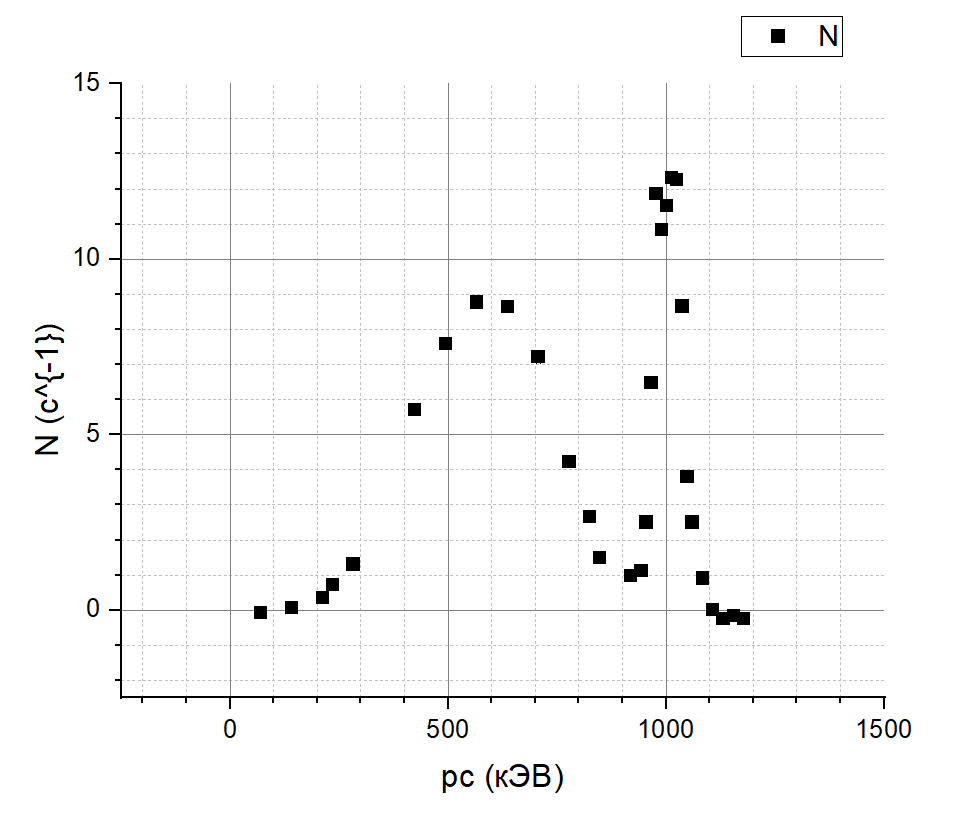
\includegraphics[width=0.9\textwidth]{gr1}
\ECaption{График спетра $N(pc)$. Из эмпирических соображений, конверсионный пик $\beta$-распада на этом спектрометре наблюдается при величине тока в 4.3 А, или 1013.5 кэВ.}
\end{center}
\end{figure}

Аналогично можно получить спектр $N$ в зависимости от энергии $E$, зная энергию конверсии 634 кэВ. Зная эти соотношения становится возможным построить график Ферми. Для этого получим уравнение графика из (2)-(4):

\begin{equation}
\frac{\sqrt{N(p)}}{p^{3/2}} \approx E_{max} - E.
\end{equation}

График Ферми показан на рис 4.

\begin{figure}[h]
\begin{center}
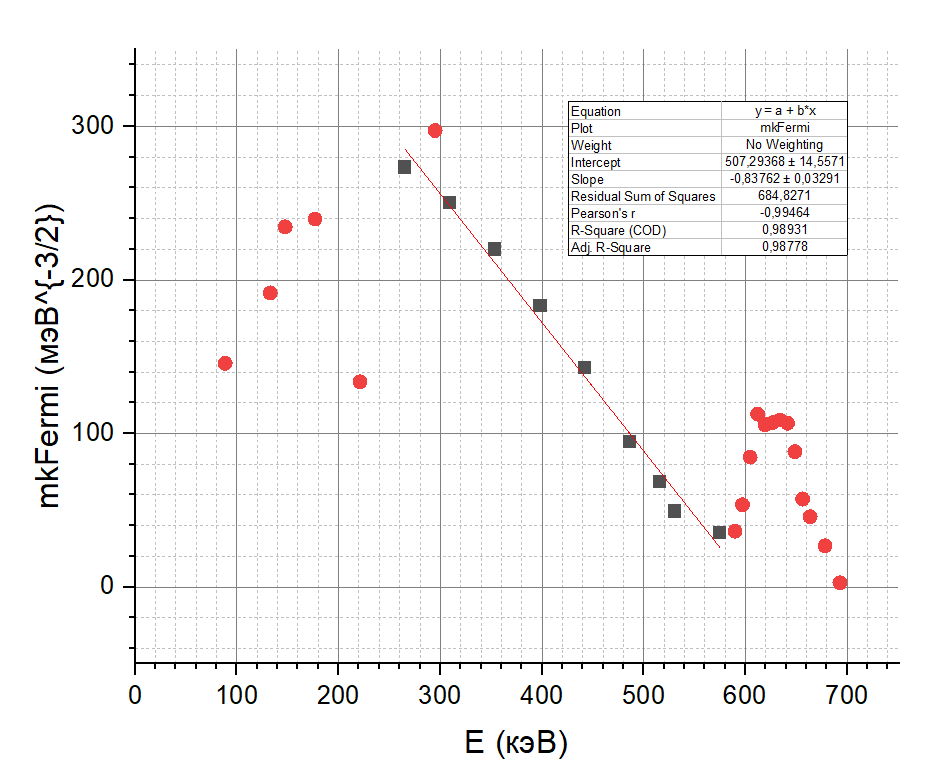
\includegraphics[width=0.9\textwidth]{gr2}
\ECaption{График Ферми. Линеаризация проходила по точкам, обозначенным черным. Эти точки получились из преобразования убывающей части исходного спектра.}
\end{center}
\end{figure}

Исходя из графика получаем максимальную энергию электрона в этом эксперименте:
\[E_{\text{max}} = 604 \pm 40 \text{ кэВ.}\]

\section*{Вывод}
В результате измерения спектра $\beta$-частиц, и последующей его обработкой с помощью точного метода графиков Ферми, была получена мансимальная энергия электрона в этом эксперименте. Она оказалась ниже, чем энергия конверсионных атомов, что объясняет то, что конверсионный пик был отделен от основного спектра. В таких условиях получить значение с приемлимой точностью можно лишь с помощью графиков Ферми. 





























\end{document}